% \documentclass{book}

\documentclass[12pt]{article}
\usepackage[pdfborder={0 0 0.5 [3 2]}]{hyperref}%
\usepackage[left=1in,right=1in,top=1in,bottom=1in]{geometry}%
\usepackage[shortalphabetic]{amsrefs}%
\usepackage{amsmath}
\usepackage{enumerate}
\usepackage{enumitem}
\usepackage{amssymb}                
\usepackage{amsmath}                
\usepackage{amsfonts}
\usepackage{amsthm}
\usepackage{bbm}
\usepackage[table,xcdraw]{xcolor}
\usepackage{tikz}
\usepackage{float}
\usepackage{booktabs}
\usepackage{svg}
\usepackage{mathtools}
\usepackage{cool}
\usepackage{url}
\usepackage{graphicx,epsfig}
\usepackage{makecell}
\usepackage{array}
\setlength\extrarowheight{25pt}

\graphicspath{ {images/} }

\begin{document}

\title{}
\author{\vspace{-10ex} }

\begin{center}
{\LARGE APMA 1650 -- Homework 1}\\
\vspace{5mm}
{\large Due Tuesday, July 5, 2016}\\
\vspace{5mm}
Homework is due during class or by 3:45 pm in the homework drop box in 182 George St.\\
Show all of your work used in deriving your solutions.
\end{center}

\begin{enumerate}
\item Suppose you flip a fair coin 50 times. Answer the following questions. You may leave the answers in terms of binomial coefficients and exponents, i.e. you don't have to expand out all the things.
\begin{enumerate}
\item What is the size of the sample space for this experiment, i.e. how many outcomes are possible?
\item What is the probability that you flip exactly 10 heads?
\item What is the probability that you flip at least 10 heads?
\item What is the probability that you never flip two heads in a row or two tails in a row?
\end{enumerate}

\item You are performing an experiment in which you survey $n$ randomly-selected people and record their birthday. Assume that there are only 365 possible birthdays, i.e. ignore leap year. Also assume that the probability of having any birthday is equally likely. You may leave the first two parts in terms of binomial coefficients and exponents, but I want a specific number for $n$ in the third part.
\begin{enumerate}
\item What is the size of the sample space for this experiment, i.e. how many outcomes are possible?
\item Take $n = 5$. What is the probability that each of the 5 people has a different birthday?
\item What is the smallest value of $n$ such that the probability is at least 0.5 that at least two people share a birthday? (This may take a little guesswork with a calculator, but I promise it is not too bad.)
\end{enumerate}

\item You enlist a friend from materials science to construct a very special unfair six-sided die. The die looks like a standard die, i.e. it it cubical and has the numbers 1, 2, 3, 4, 5, and 6 on its faces. On this die, the probability of rolling any number is directly proportional to that number. For example, you are twice as likely to roll a 6 as a 3. 
\begin{enumerate}
\item What is the probability of rolling each of the six numbers?
\item What is the probabiltiy of rolling an odd number?
\end{enumerate}

\item Consider the grid of points shown below. You start at (0, 0) and take one step either up or to the right with each move. You keep moving until you reach (10, 10). You can never leave the grid. For example, if you reach the point (4, 10), you can only move to the right from that point onwards. Assume that each possible path is equally likely. Answer the following questions. You may leave the answers in terms of binomial coefficients and exponents.
\begin{enumerate}
\item What is the size of the sample space, i.e. how many possible paths are there from (0, 0) to (10, 10)?
\item What is the probability that a path passes through (5, 5)?
\end{enumerate}
\begin{figure}[H]
\centering
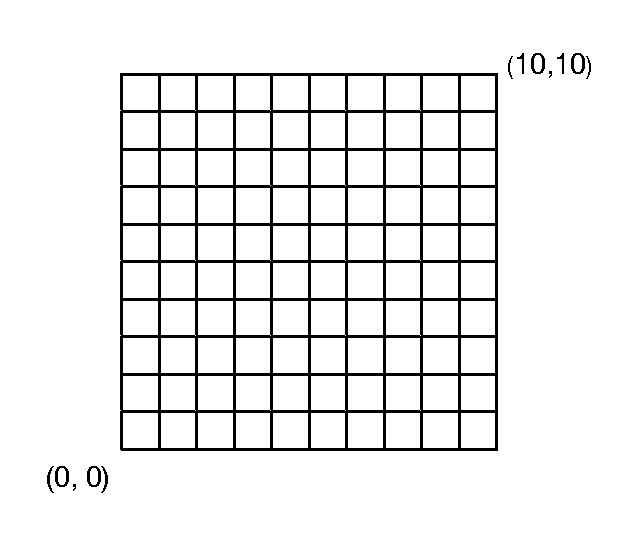
\includegraphics[width=10cm]{grid.eps}
\end{figure}

\item Powerball is an American lottery game offered by 44 states (including Rhode Island). To play the game, you select 5 distinct numbers from a set of 69 white balls (numbered 1 - 69) and one number from a set of 26 red Powerballs (numbered 1 - 26). In each drawing, five white balls and one red Powerball are selected\footnote{If you Google ``Powerball'', today's numbers are displayed at the top of the search results. In asking this question, the instructor is not condoning playing Powerball. }. The order of the white balls does not matter. (In the official Powerball drawing, the white balls are listed in ascending order.) 
\begin{enumerate}
\item You win the jackpot if you match all 5 white balls and the Powerball. What is the probability that you win the jackpot?
\item If you match all 5 white balls but do not match the Powerball, you win \$1,000,000. What is the probability that this occurs?
\item If you match the Powerball but do not match \emph{any} of the white balls, you win \$4. What is the probability that this occurs?
\item If you match \emph{exactly} 3 white balls (so you don't match the other two balls) and the Powerball, you win \$100. What is the probability that this occurs?
\end{enumerate}

\end{enumerate}
\end{document}

